\documentclass[11pt]{article}

% ACL style
\usepackage[preprint]{acl}

% Fonts
\usepackage[T1]{fontenc}
\usepackage[utf8]{inputenc}
\usepackage{times}
\usepackage{inconsolata}

% Packages
\usepackage{graphicx}
\usepackage{booktabs}
\usepackage{multirow}
\usepackage[normalem]{ulem}
\usepackage{amsmath}

\graphicspath{{../llm2seq/figures/}{llm2seq/figures/}}

\title{LLM2Seq: Task-Specific Encoder-Decoder Adaptation for Abstractive Summarization}

\author{
Giang-Bien Kieu \\
Hanoi University of Science and Technology\\
HUST, Vietnam\\
\texttt{bienkieugiang@gmail.com}
\And
Xuan-Dung Doan\\
Viettel Artificial Intelligence Center\\
Viettel Group, Vietnam\\
\texttt{dungdx4@viettel.com.vn}
}

\begin{document}
\maketitle

\begin{abstract}
Decoder-only language models are powerful generators, but their causal formulation is not always the most efficient interface for long-input sequence-to-sequence tasks such as abstractive summarization.
Recent work on latent context compression shows that encoder-decoder interfaces can reduce long-context inference cost by mapping raw tokens into compact continuous memories.
In this work, we study a different point in this design space: task-specific encoder-decoder adaptation for summarization under limited training resources.
We present LLM2Seq, a framework that repurposes a decoder-only model as the source encoder and connects it to a lightweight Transformer decoder through a gated residual adaptor.
Unlike general-purpose latent context compressors that aggressively reduce input length, LLM2Seq preserves token-level source evidence and learns a summarization-oriented memory interface for cross-attentive generation.
On WikiLingua, our Qwen-based LLM2Seq model achieves 54.01 ROUGE-1, 20.83 ROUGE-2, and 31.83 ROUGE-L, approaching a larger T5Gemma-2-1B-1B LoRA baseline on ROUGE-1 while producing summaries much closer to the reference length.
We further investigate multi-token prediction with verified decoding for encoder-decoder summarization.
The Qwen variant obtains a measured 1.17x token-per-second speedup with small ROUGE changes, while the Llama variant shows that higher accepted-token rates do not necessarily translate into end-to-end speedups when verification overhead dominates.
These results position LLM2Seq as a practical task-specific alternative to large-scale context compression for long-input summarization.
\end{abstract}

\section{Introduction}
\label{sec:introduction}

Long-input summarization sits between two needs.
The model must read a long source document.
It must also generate a short and faithful target.
Decoder-only LLMs are strong generators \citep{brown2020language,dubey2024llama3,yang2024qwen2}, but their left-to-right interface is not naturally built around this separation.
Encoder-decoder models are a better structural fit because the encoder first builds source representations and the decoder then generates through cross-attention \citep{sutskever2014sequence,bahdanau2015neural,vaswani2017attention}.
This is why T5, BART, and mT5 remain strong sequence-to-sequence baselines \citep{raffel2020t5,lewis2020bart,xue2021mt5}.

Recent work has reopened the encoder-decoder design space for modern LLMs.
LLM2Vec shows that decoder-only LLMs can be converted into strong bidirectional encoders \citep{behnamghader2024llm2vec}.
LaMaTE studies LLM encoders for machine translation \citep{luo2025lamate}.
T5Gemma builds encoder-decoder models from Gemma-style components \citep{zhang2025t5gemma2}.
At the same time, Latent Context Language Models (LCLMs) show that encoder-decoder compressors can map long contexts into fewer latent tokens and improve the accuracy-efficiency frontier for long-context inference \citep{li2026contextcompression}.

This paper studies a different operating point.
LLM2Seq is not a general context compressor.
It does not compress every $N$ tokens into one reusable latent token.
Instead, it keeps high-resolution token-level source memory and learns a summarization-specific bridge from decoder-only representations to a cross-attentive decoder.
The goal is not to beat LCLM at general context compression.
The goal is to ask whether a decoder-only LLM representation can be turned into a practical encoder-decoder summarizer with task-level training.

Our contributions are:
\begin{itemize}
    \item We formulate LLM2Seq as a task-specific alternative to general latent context compression for abstractive summarization.
    \item We instantiate a gated residual adaptor that converts decoder-only encoder states into cross-attendable source memory for a lightweight Transformer decoder.
    \item We compare Llama- and Qwen-based encoders under the same decoder and adaptor design, showing that encoder choice strongly affects summarization quality.
    \item We evaluate MTP with verified decoding in an encoder-decoder summarization setting and show that real speedup depends on system overhead, not only on accepted draft tokens.
\end{itemize}

\section{Related Work}
\label{sec:related}

\paragraph{Encoder-decoder generation.}
Sequence-to-sequence learning first used recurrent encoders and decoders \citep{sutskever2014sequence}.
Attention let the decoder select source information during generation \citep{bahdanau2015neural}.
The Transformer made self-attention the standard architecture \citep{vaswani2017attention}.
T5 frames NLP tasks as text-to-text generation \citep{raffel2020t5}.
BART uses denoising pretraining for generation and summarization \citep{lewis2020bart}.
mT5 extends this recipe to multilingual settings \citep{xue2021mt5}.

\paragraph{Repurposing LLMs as encoders.}
LLM2Vec converts decoder-only LLMs into bidirectional text encoders \citep{behnamghader2024llm2vec}.
GRIT also shows that generative models can learn useful representations \citep{muennighoff2024grit}.
LaMaTE studies large language models as encoders for machine translation \citep{luo2025lamate}.
Our work follows this line, but uses the repurposed encoder for long-input summarization.

\paragraph{Latent context compression.}
End-to-End Context Compression at Scale introduces LCLMs, a family of encoder-decoder compressors trained at scale for long-context inference \citep{li2026contextcompression}.
LCLMs map long token sequences into shorter latent sequences at fixed compression ratios such as 1:4, 1:8, and 1:16.
They train 0.6B-encoder and 4B-decoder models on more than 350B tokens and optimize a Pareto frontier over accuracy, time-to-first-token, and memory.
LLM2Seq is complementary.
It uses an encoder-decoder latent memory interface, but it is task-specific and keeps token-level memory for summarization.

\paragraph{Efficient decoding.}
Speculative decoding drafts tokens and verifies them with a target model \citep{leviathan2023speculative}.
Blockwise parallel decoding predicts several future tokens in one step \citep{stern2018blockwise}.
Medusa adds extra decoding heads to accelerate LLM inference \citep{cai2024medusa}.
Multi-token prediction trains models to predict future tokens directly \citep{gloeckle2024mtp}.
MTP-D studies self-distillation for MTP heads \citep{zhao2026mtpdistill}, following the broader idea of knowledge distillation \citep{hinton2015distilling}.
DeepSeek-V3 also uses MTP-style training in a large-scale LLM system \citep{deepseekai2024deepseekv3}.

\section{LLM2Seq and Context Compression}
\label{sec:lclm-relation}

LLM2Seq is closely related to recent encoder-decoder context compression models, especially LCLMs.
Both approaches replace the standard decoder-only interface with an encoder-decoder-style latent memory interface.
However, they target different regimes.

\begin{table*}[t]
\centering
\small
\begin{tabular}{p{0.18\linewidth}p{0.36\linewidth}p{0.36\linewidth}}
\toprule
Axis & LCLM / End-to-End Context Compression & LLM2Seq \\
\midrule
Goal & General long-context compression for LLM inference & Task-specific abstractive summarization \\
Memory & Compress $N$ source tokens into fewer latent tokens & Preserve token-level source memory \\
Ratio & Fixed ratios such as 1:4, 1:8, and 1:16 & No hard token compression ratio \\
Training & Continual pretraining at large scale & WikiLingua task training with LoRA \\
Decoder & Large decoder preserves broad capability & Lightweight decoder focuses on summaries \\
Metrics & TTFT, peak memory, long-context accuracy & ROUGE, length, latency, token/s \\
\bottomrule
\end{tabular}
\caption{LLM2Seq is not designed to beat LCLM at general context compression. It studies a task-specific point in the same encoder-decoder memory design space.}
\label{tab:lclm-compare}
\end{table*}

LCLM is a general compressor.
It is designed so a decoder can consume compressed context and still preserve broad language-model capabilities.
LLM2Seq instead targets one task.
It keeps a high-resolution source memory because summarization needs source evidence.
A faithful summary often depends on small local details.
Aggressive latent compression may be useful, but it is a different question from the one studied here.

This framing also limits our claims.
We do not claim a new general-purpose context compressor.
We claim that decoder-only representations can be adapted into a cross-attentive summarization memory, and that the quality, length, and latency trade-offs can be measured under practical training budgets.

\section{Method}
\label{sec:method}

\begin{figure}[t]
\centering
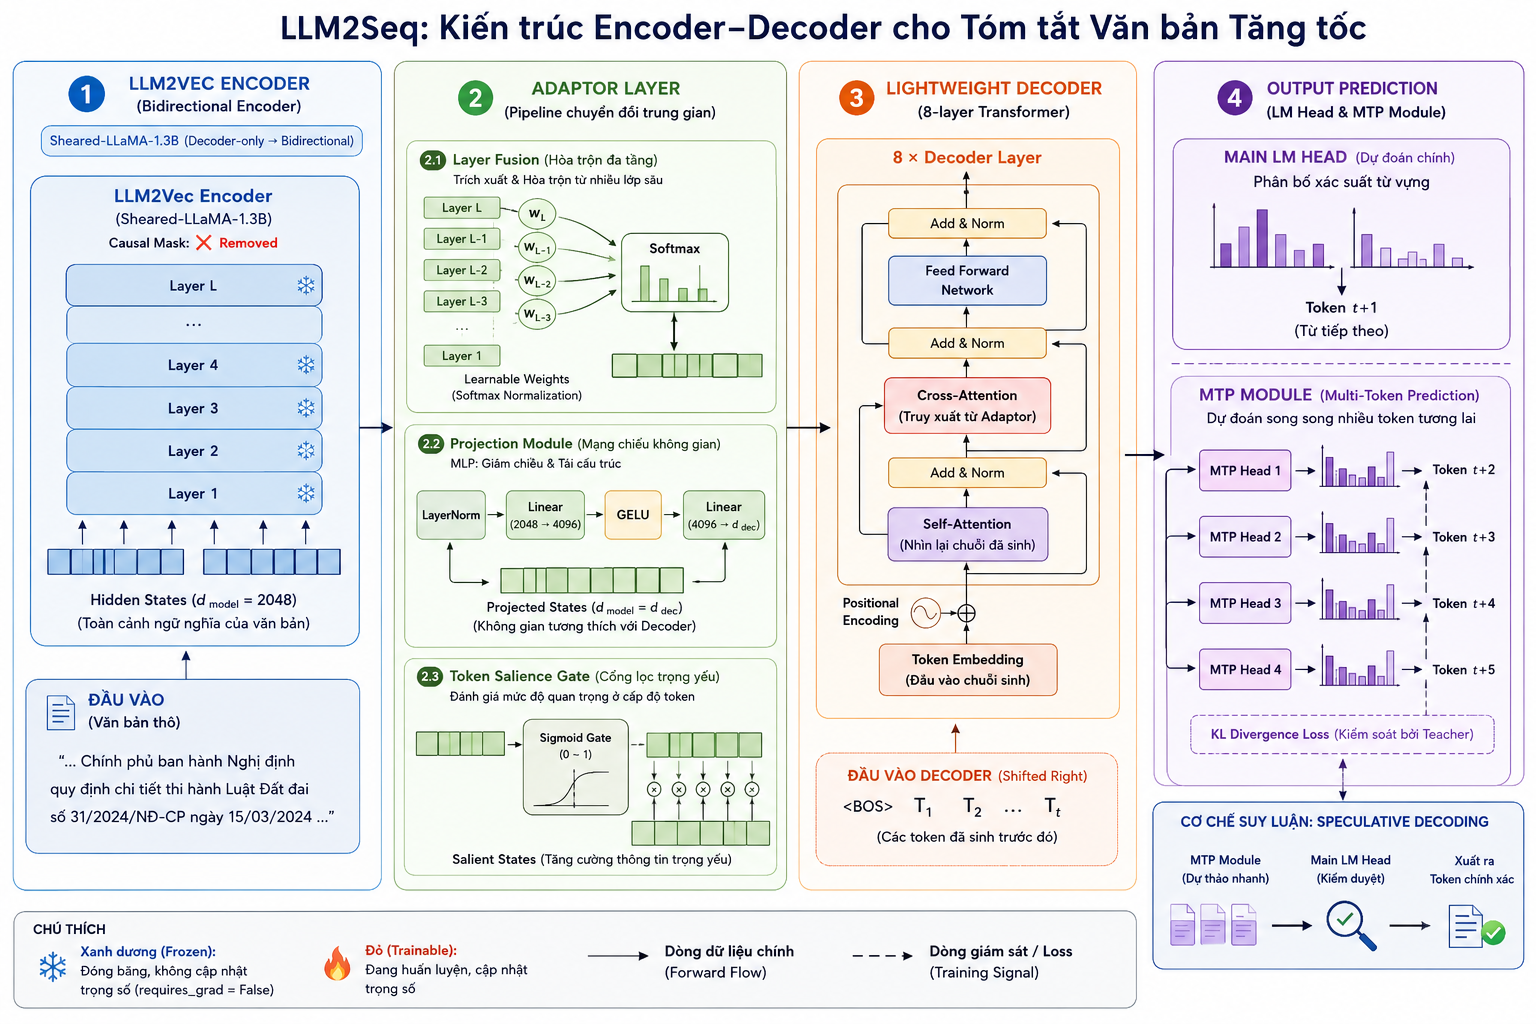
\includegraphics[width=\linewidth]{image.png}
\caption{LLM2Seq converts a decoder-only model into a source encoder and connects it to a lightweight decoder through a gated residual adaptor.}
\label{fig:architecture}
\end{figure}

\subsection{LLM Encoder}

The encoder starts from a decoder-only or embedding-oriented LLM.
For the Llama variant, we use \texttt{LLM2Vec-Sheared-LLaMA-mntp}.
For the Qwen variant, we use \texttt{Qwen3-Embedding-0.6B}.
The model reads the source document and outputs contextual token states.
The WikiLingua setup uses source lengths up to 3,072 tokens and target lengths up to 384 tokens.

Full encoder fine-tuning is expensive.
Phase 2 therefore uses LoRA on the encoder \citep{hu2022lora}.
This keeps the training budget small compared with large-scale context compression pretraining.

\subsection{Gated Residual Adaptor}

The adaptor maps encoder states into decoder memory.
It has layer fusion, a gated residual projection, a token salience gate, an EncStack, and 16 global memory tokens.
Layer fusion combines information from multiple encoder layers, which is useful because different Transformer layers carry different levels of information \citep{wang2019deeptransformer}.
The salience gate and memory tokens are designed to help the decoder focus on the source content.

We treat the adaptor as a design choice, not as a fully isolated proven contribution.
The current snapshot does not include a complete per-component ablation.
This is why our claims about the adaptor stay conservative.

\subsection{Lightweight Decoder}

The decoder is an 8-layer Transformer decoder with hidden size 1024, 16 attention heads, and a 4096-dimensional feed-forward layer.
It uses masked self-attention over target tokens and cross-attention over adapted source memory.
The decoder is smaller than the encoder so generation remains relatively cheap.

\subsection{MTP with Verified Decoding}

Phase 3 adds cascaded MTP heads.
We use $K=4$ draft heads.
The main summarization path is frozen.
Only the MTP module is trained.
The loss is:
\[
\mathcal{L}
= \lambda_{CE}\mathcal{L}_{CE}
+ \lambda_{KL}\mathcal{L}_{KL}.
\]
The current setting uses $\lambda_{CE}=0.6$ and $\lambda_{KL}=0.2$.
The KL term starts after 20\% of training and ramps until 50\%.
The head weights are $[1.0, 0.8, 0.5, 0.25]$.

At inference time, MTP drafts future tokens and the main head verifies them.
This can reduce decoding steps.
But it also adds verifier cost.
The real metric is wall-clock throughput, not only accepted tokens per step.

\section{Experiments}
\label{sec:experiments}

\subsection{Dataset and Baselines}

We evaluate on WikiLingua, a multilingual abstractive summarization dataset built from WikiHow articles \citep{ladhak2020wikilingua}.
The processed English split has 13,999 training examples, 1,680 validation examples, and 3,901 test examples.

We compare:
\begin{itemize}
    \item \textbf{LLM2Seq-Llama}: LLM2Vec-Sheared-LLaMA encoder with the LLM2Seq decoder.
    \item \textbf{LLM2Seq-Qwen}: Qwen3-Embedding-0.6B encoder with the same decoder and adaptor.
    \item \textbf{T5Gemma}: T5Gemma-2-1B-1B fine-tuned with LoRA \citep{zhang2025t5gemma2}.
\end{itemize}

All models use greedy decoding, repetition penalty, and no-repeat trigram blocking.

\subsection{Metrics}

We report ROUGE \citep{lin2004rouge}, BLEU \citep{post2018call}, chrF, length statistics, and speed.
For speed, we use generated tokens per second and mean latency from the evaluation logs.
For length, we report mean predicted words and too-long rate.
This matters because a model can improve overlap by generating longer summaries.

\section{Results}
\label{sec:results}

\subsection{Quality and Length}

Table~\ref{tab:main-results} shows the main WikiLingua results.
T5Gemma has the best ROUGE-2 and ROUGE-L.
LLM2Seq-Qwen is close on ROUGE-1 and much stronger than LLM2Seq-Llama.
It also produces summaries closer to the reference length than T5Gemma.

\begin{table*}[t]
\centering
\small
\begin{tabular}{lrrrrrrrr}
\toprule
Model & R-1 & R-2 & R-L & BLEU & chrF & Pred. words & Ref. words & Too-long \\
\midrule
LLM2Seq-Llama & 48.36 & 15.54 & 29.05 & 3.43 & 15.45 & 29.10 & 51.86 & 5.46 \\
LLM2Seq-Qwen & 54.01 & 20.83 & 31.83 & 7.58 & 24.66 & 58.31 & 51.86 & 35.79 \\
T5Gemma-2-1B-1B & \textbf{54.24} & \textbf{27.42} & \textbf{33.89} & \textbf{8.84} & \textbf{33.60} & 90.89 & 51.86 & 68.03 \\
\bottomrule
\end{tabular}
\caption{WikiLingua test results. Too-long is a percentage. T5Gemma has the best overlap scores, but it generates much longer summaries.}
\label{tab:main-results}
\end{table*}

The Llama variant under-generates.
Its mean output is only 29.10 words.
The Qwen variant is closer to the reference mean length, with 58.31 words versus 51.86 reference words.
T5Gemma is strongest by ROUGE, but its mean output is 90.89 words and its too-long rate is 68.03\%.
Therefore, the fair conclusion is not that LLM2Seq beats T5Gemma.
The conclusion is that LLM2Seq-Qwen is competitive on ROUGE-1 and offers a more compact summarization behavior.

\subsection{Autoregressive Speed}

Table~\ref{tab:speed} shows autoregressive decoding speed.
T5Gemma is fastest in this setup.
This is an important baseline because it prevents overclaiming LLM2Seq as generally faster.

\begin{table}[t]
\centering
\small
\begin{tabular}{lrr}
\toprule
Model & tok/s & Mean latency \\
\midrule
LLM2Seq-Llama & 114.74 & 0.697s \\
LLM2Seq-Qwen & 95.87 & 0.779s \\
T5Gemma-2-1B-1B & \textbf{257.70} & \textbf{0.412s} \\
\bottomrule
\end{tabular}
\caption{Autoregressive decoding speed on WikiLingua.}
\label{tab:speed}
\end{table}

\subsection{MTP: Accepted Tokens Are Not Throughput}

Table~\ref{tab:mtp-results} gives the main MTP result.
This is the clearest system-level finding.
MTP reduces decoding steps for both encoders.
But only Qwen turns that into real throughput.

\begin{table*}[t]
\centering
\small
\begin{tabular}{lrrrrrrr}
\toprule
Model & Mode & tok/s & Speedup & Tokens/step & Mean lat. & R-1 & R-L \\
\midrule
Llama & AR & 114.74 & 1.00x & 1.00 & 0.697s & 48.36 & 29.05 \\
Llama & MTP & 73.14 & 0.64x & 2.45 & 1.094s & 48.36 & 29.05 \\
Qwen & AR & 95.87 & 1.00x & 1.00 & 0.779s & 54.01 & 31.83 \\
Qwen & MTP & \textbf{111.71} & \textbf{1.17x} & 2.30 & \textbf{0.662s} & 53.90 & 31.64 \\
\bottomrule
\end{tabular}
\caption{Verified MTP results. AR means autoregressive decoding. MTP improves tokens per step for both encoders, but real throughput improves only for Qwen.}
\label{tab:mtp-results}
\end{table*}

The Llama result is negative but useful.
It emits 2.45 tokens per decoding step, yet speed drops to 0.64x.
The Qwen result is better.
It reaches 1.17x measured token-per-second speedup and lowers mean latency from 0.779s to 0.662s.
ROUGE changes are small: ROUGE-1 drops by 0.11 and ROUGE-L drops by 0.19.

This means MTP should not be evaluated only by accepted-token rate.
The verifier, tensor control flow, and implementation overhead decide whether accepted tokens become real speed.

\section{Discussion}
\label{sec:discussion}

\paragraph{What LLM2Seq contributes.}
The contribution is not ``we invented encoder-decoder LLMs.''
That space already includes LLM2Vec, LaMaTE, T5Gemma, and LCLM.
The contribution is narrower.
LLM2Seq studies task-specific high-resolution memory adaptation for summarization.
It keeps source evidence as token-level memory, trains with limited task data, and measures quality, length, and decoding speed together.

\paragraph{Why Qwen matters.}
Changing the encoder from Llama to Qwen improves ROUGE-1 from 48.36 to 54.01 and ROUGE-L from 29.05 to 31.83 under the same LLM2Seq decoder and adaptor design.
This suggests that the encoder representation is a major factor.
The adaptor can only expose information that exists in the source encoder states.

\paragraph{Why T5Gemma is still strong.}
T5Gemma is a native encoder-decoder model and a strong baseline.
It wins ROUGE-2 and ROUGE-L.
At the same time, it generates much longer summaries.
A stronger future comparison should control output length directly.
For example, T5Gemma could be evaluated under the same target length budget as LLM2Seq-Qwen.

\paragraph{Why adaptor claims must stay conservative.}
The adaptor is plausible and useful in the current system.
But the current result files do not include enough ablations to prove each component.
A clean next experiment should compare linear projection, MLP adaptor, MLP plus EncStack, and the full gated residual adaptor.
Another direct experiment should test LCLM-style block compression, such as mean-pooling encoder states by 4, 8, or 16 tokens before the decoder.

\paragraph{Why MTP speedup is limited.}
For Qwen, MTP emits 2.30 tokens per step but gives only 1.17x real speedup.
This gap is expected because verified decoding adds work.
For Llama, the overhead dominates completely.
Future work should fuse verification, use \texttt{torch.compile}, or move the hot path into an optimized runtime such as vLLM.
Deployment-oriented methods such as SmoothQuant may also help under memory limits \citep{xiao2023smoothquant}.

\section{Conclusion}
\label{sec:conclusion}

LLM2Seq is best understood as a task-specific encoder-decoder adaptation method for long-input summarization.
It is related to latent context compression, but it targets a different regime.
Instead of compressing arbitrary context into reusable short latent sequences, it preserves source evidence and learns a summarization-oriented memory interface.

On WikiLingua, the Qwen-based LLM2Seq model is competitive with T5Gemma on ROUGE-1 and produces summaries closer to the reference length.
MTP gives a real 1.17x speedup for Qwen, but the Llama result shows that accepted draft tokens are not the same as throughput.
The next step is clear: add compression and adaptor ablations, then optimize verified decoding.

\section*{Limitations}

The report uses completed metrics available in the current project snapshot.
It does not include a full adaptor ablation or an LCLM-style block-compression baseline.
It also does not claim general-purpose context compression.
The MTP results measure the current implementation, not a fused serving runtime.

\bibliography{custom}

\end{document}
